\documentclass{article}
\usepackage{amsmath}
\usepackage{mathtools}
\usepackage{gensymb}
\usepackage[a4paper,inner=1.5cm,outer=1.5cm,top=2cm,bottom=0.5cm]{geometry} 
\usepackage{xcolor}                    
\usepackage{tikz}                           
\usepackage{multicol}
\usepackage{pgfplots}
\usetikzlibrary{calc}
\usetikzlibrary{intersections}
\usetikzlibrary{intersections,calc,angles,quotes}
\usetikzlibrary{shapes,arrows,positioning,decorations.pathreplacing,calc}
\usetikzlibrary{calc,angles,positioning,intersections,quotes,decorations.markings}
\usepackage{tkz-euclide}
\usetikzlibrary{backgrounds}
\usetikzlibrary{calc,through}
\usetikzlibrary{angles}
\usetikzlibrary{fadings}
\usetikzlibrary{shapes.geometric}
\usetikzlibrary{shapes.symbols}
\usepackage{draftwatermark}
\usepackage{mathptmx}

\SetWatermarkText{\textcolor{black!30}{Mathema Shukur}}
\SetWatermarkFontSize{2 cm}
\usepackage[utf8]{inputenc}
\usepackage{fontspec}

\setmainfont{[Kalpurush.ttf]}
\newfontface{\en}{[Arial.ttf]} %%this is optional, if you want to use a secondary font. Any english font is supported
\newlength\Radius
\setlength\Radius{4cm}
\begin{document} 
	\Large
	\textcolor{red}{Welcome To} 
	\\
	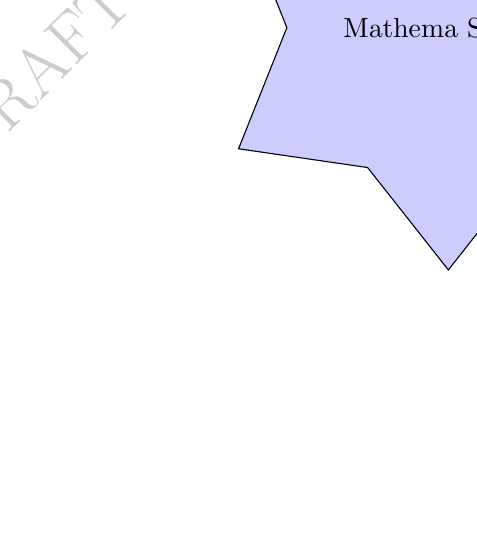
\begin{tikzpicture}
		\tikz \node [fill=blue!20,star,star points=6,draw] {Mathema Shukur };
	\end{tikzpicture}
	\\
	যাদের জন্যে প্রযোজ্যঃ  	\textcolor{magenta}{একাদশ ও দ্বাদশ শ্রেণীর শিক্ষার্থী} \\
	বিষয়ঃ \textcolor{magenta}{উচ্চতর গণিত ১ম পত্র} \\
	অধ্যায়ঃ \textcolor{magenta}{৩-সরলরেখা}\\ 
	Subtopicঃ  \textcolor{magenta}{ $ax+by+c=0$ এর লম্ব রেখার সমীকরণ নির্ণয় কর }\\
	\\
	\textcolor{blue}{$ax+by+c=0$ এর লম্ব রেখার সমীকরণ   $bx-ay+k=0$}\\
	\\
(১) মূল সমীকরণের $x$ এর সহগ মডেল সমীকরণে হবে $y$ এর সহগ \\
	\\
(২) মূল সমীকরণের $y$ এর সহগ মডেল সমীকরণে হবে $x$ এর সহগ \\
		\\ 
(৩) যেকোনো একটি সহগের চিহ্ন পরিবর্তন হবে \\
\\
(৪) এ ক্ষেত্রে ধ্রুবক পদ পরিবর্তিত হবে \\ 
\\
\begin{multicols}{2}
	\begin{align*}
	\textcolor{blue}{(+a)}x+	\textcolor{red}{(+b)}y+c&=0\\
	\\
	\textcolor{red}{(+b)}x+	\textcolor{blue}{(-a)}y+k&=0\\
	\\
	bx-ay+k&=0
\end{align*}
\\
বিকল্প পদ্ধতি\\ 
\begin{align*}
	\textcolor{blue}{(+a)}x+	\textcolor{red}{(+b)}y+c&=0\\
	\\
	\textcolor{red}{(-b)}x+	\textcolor{blue}{(+a)}y+k&=0\\
	\\
	-bx+ay+k&=0
\end{align*}
\end{multicols}	
\vspace{2cm}
	 যশোর বোর্ড-২০২১\\ 
	$(1,2)$ বিন্দুগামী এবং $3x-4y+8=0$ রেখাটির উপর লম্ব রেখার সমীকরণ নির্ণয় কর \\
	\\
	\textcolor{red}{step-01}\\
	\begin{align*}
		3x-4y+8&=0\\
		\\
		\textcolor{blue}{(+3)}x+	\textcolor{red}{(-4)}y+8&=0\\
		\\
		\textcolor{red}{(+4)}x+	\textcolor{blue}{(+3)}y+k&=0\\
		\\
	4x+3y+k&=0
	\end{align*}\\ 
	\\
	\textcolor{red}{step-02}	$4x+3y+k=0$ রেখাটি $(1,2)$ বিন্দুগামী \\
	\\
	\begin{align*}
			4x+3y+k&=0\\
		\\
		4(1)+3(2)+k&=0\\
		\\
		10+k&=0\\
		\\
		k&=-10
	\end{align*}
	\\
	$(1,2)$ বিন্দুগামী এবং $3x-4y+8=0$ রেখাটির উপর লম্ব রেখার সমীকরণ $4x+3y-10=0$\\
	\\
	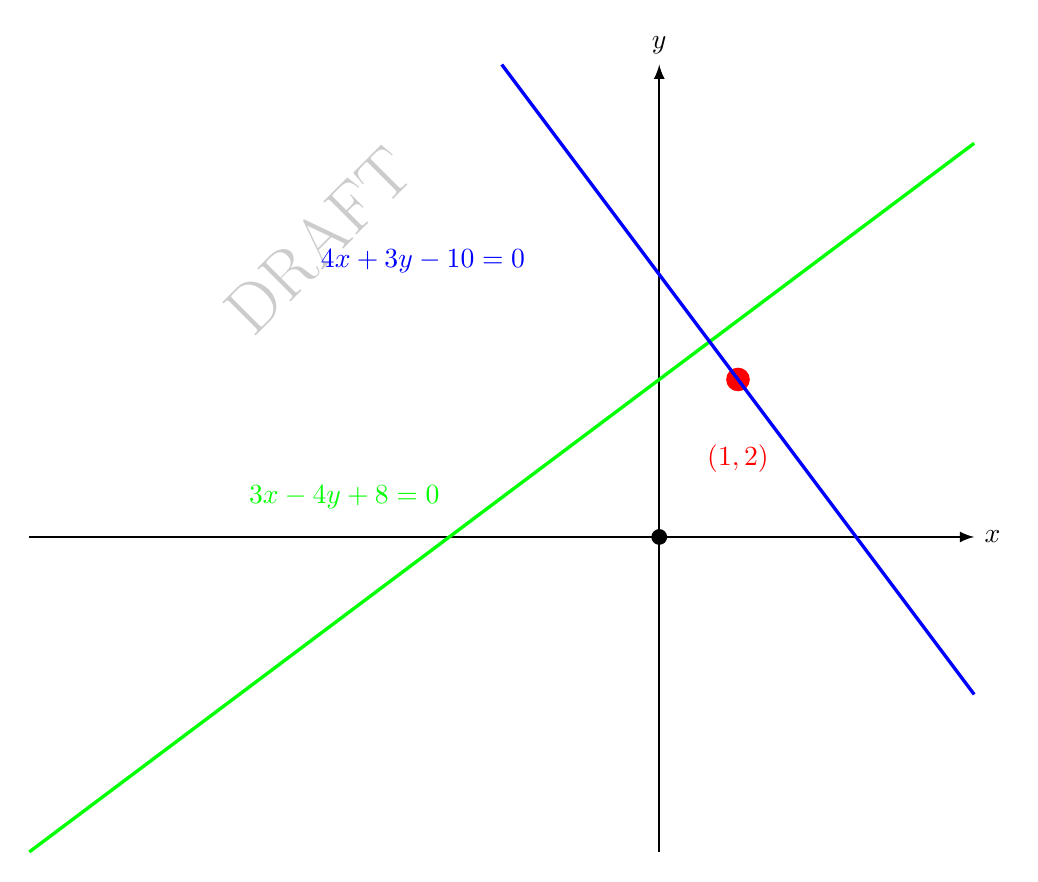
\begin{tikzpicture}[transform shape,scale=1]
		\draw [-latex,thick](-8,0) -- (4,0) node[right] {$x$} coordinate(x axis);
		\draw [-latex,thick](0,-4) -- (0,6) node[above] {$y$} coordinate(y axis);
		\fill[black] (0,0) circle (1 mm);
		\fill[red] (1,2) circle (1.5 mm);
		\node at (-3,3.5) {$\textcolor{blue}{4x+3y-10=0}$};	
		\node at (-4,0.5) {$\textcolor{green}{3x-4y+8=0}$};	
		\node at (1,1) {$\textcolor{red}{(1,2)}$};	
		\draw[very thick,green] (-8,-4)--(4,5);	
		\draw[very thick,blue] (-2,6)--(4,-2);	
	\end{tikzpicture}
\\
	ময়মনসিংহ বোর্ড-২০২১\\
	$3x+8y-24=0$ রেখাটির উপর লম্ব এবং $(3,8)$ বিন্দুগামী সরলরেখার সমীকরণ নির্ণয় কর \\
	\\ 
		\textcolor{red}{step-01}\\
	\begin{align*}
	3x+8y-24&=0\\
		\\
		\textcolor{blue}{(+3)}x+\textcolor{red}{(+8)}y-24&=0\\
		\\
		\textcolor{red}{(+8)}x+	\textcolor{blue}{(-3)}y+k&=0\\
		\\
		8x-3y+k&=0
	\end{align*}\\ 
	\\
	\textcolor{red}{step-02}	$8x-3y+k=0$ রেখাটি $(3,8)$ বিন্দুগামী \\
	\\
	\begin{align*}
	8x-3y+k&=0\\
		\\
		8(3)-3(8)+k&=0\\
		\\
		24-24+k&=0\\
		\\
		k&=0
	\end{align*}
	\\
	$3x+8y-24=0$ রেখাটির উপর লম্ব এবং $(3,8)$ বিন্দুগামী  রেখার সমীকরণ $8x-3y=0$\\
	\\
	\begin{tikzpicture}[transform shape,scale=1]
		\draw [-latex,thick](-8,0) -- (11,0) node[right] {$x$} coordinate(x axis);
		\draw [-latex,thick](0,-8) -- (0,8) node[above] {$y$} coordinate(y axis);
		\fill[black] (0,0) circle (1 mm);
		\fill[red] (3,8) circle (1.5 mm);
		\node at (3,3.5) {$\textcolor{blue}{8x-3y=0}$};	
		\node at (-4,3.5) {$\textcolor{green}{3x+8y-24=0}$};	
		\node at (2,7.5) {$\textcolor{red}{(3,8)}$};	
		\draw[very thick,green] (-8,6)--(11,-1.1);	
		\draw[very thick,blue] (3,8)--(-3,-8);	
	\end{tikzpicture}
	\\
	\vspace{4cm}
	\\
	\textcolor{red}{$ax+by+c=0$ সরলরেখার  লম্ব সরলরেখা যা $(\alpha, \beta )$ বিন্দুগামী এরুপ সরলরেখার সমীকরণ  $bx-ay=b\alpha-a\beta$}\\
	\\ 
রাজশাহী বোর্ড-২০২২\\
	$(1,2)$ বিন্দুগামী $2x-3y-9=0$ রেখার উপর লম্বরেখার  সমীকরণ নির্ণয় কর \\
	\\ 
	\textcolor{red}{single step}	$2x-3y-9=0$  রেখার উপর লম্ব  এবং  $(1,2)$ বিন্দুগামী এরুপ সরলরেখার সমীকরণ \\
	\\
	$3x+2y=3(1)+2(2)=7$\\
	\\
	$3x+2y=7$\\
	\\
	\begin{tikzpicture}[transform shape,scale=1]
		\draw [-latex,thick](-3,0) -- (9,0) node[right] {$x$} coordinate(x axis);
		\draw [-latex,thick](0,-5) -- (0,8) node[above] {$y$} coordinate(y axis);
		\fill[black] (0,0) circle (1 mm);
			\fill[red] (1,2) circle (1.5 mm);
				\node at (1.7,2.5) {$\textcolor{red}{(1,2)}$};	
		\node at (-2,3.5) {$\textcolor{blue}{3x+2y-7=0}$};	
		\node at (4.5,1.5) {$\textcolor{green}{2x-3y-9=0}$};	
		\draw[very thick,green] (-3,-5)--(9,3);	
		\draw[very thick,blue] (-3,8)--(5,-4);	
	\end{tikzpicture}
	\\
	$(1,2)$ বিন্দুগামী $2x-3y-9=0$ রেখার উপর লম্বরেখার  সমীকরণ	$3x+2y=7$
\end{document}